
\documentclass[a4paper,14pt]{article}
\usepackage{natbib}
\usepackage{ucs}
\usepackage[utf8x]{inputenc}
\usepackage[T1]{fontenc}

\usepackage{graphics}
\usepackage{tipa}
\usepackage{multirow}

\begin{document}
\title{Mo oažžut dihtora hálddašit lunddolaš giela válljenvejolašvuođaid giellaoahppanproseassas? \\ Gielalaš ja pedagogalaš čuolmmat.}   
\author{Lene Antonsen, Biret Ánne Bals Baal, \\ Saara Huhmarniemi, Trond Trosterud \\ Romssa Universitehta} 
\date{} 
\maketitle
\pagenumbering{arabic}
 
\maketitle
\tableofcontents

%\subsection{Table of contents}\tableofcontents} 

\section{Álggahus}

\subsection{pedagogaglaš idea}
Prográmma galgá bagadit geavaheaddji seammá ládje go oahpaheaddji dahká.


%\subsection{VISL-prográmmat ??}
%\textbf{Oahppat grámmatihka:}\\
%Sátneluohkáid, syntávssa.


\subsection{Giellateknologiija}
- vejolaččat - Let´s Chat - multiple choice
- string match
- mo CG doaibmá
- min systema \\

Pedagogalaš prográmmain ii leat dábálaččat giellateknologiija, muhto
\begin{itemize}
\item multiple choice 
\item stringmatch, omd \textit{viesus} = 6 mearkka: v i e s u s
\end{itemize}
Giellateknologiija:
\begin{itemize}
\item analysa, omd \textit{viesus} = \textit{viessu} N Sg Loc
\end{itemize}

\subsection{Lingvisttalaš máhttu} 
Mii geavahit min máhtu:
\begin{itemize}
\item sámegiela syntávssa birra		
\item ohppiid gaskagiela birra
\end{itemize}

\subsection{Sámegiela syntáksa} 
omd. maid NP sáhttá sisttisdoallat:
\begin{itemize}
\item \small{NP $\rightarrow$ Pron A N Num Adv A CC Adv A N}  \\ 	
\textit{mu boares áhku guokte hui stuora ja hirbmat váralaš beatnaga}	
\item makkár kongruensa NP siskkobealde
\end{itemize}


\section{OAHPA-prográmmat}
- eará sámegiel. progr?
\textbf{Oahppat sámegiela:}\\
\begin{itemize}
\item \textbf{Leksa}: Sátnequiz - sámi/dáru ja dáru/sámi
\item  \textbf{Numra}: Hárjehallat loguid
\item  \textbf{Morfa}: Hárjehallat sojahit sániid, maid konteavsttas
\item  \textbf{Vasta}: Hárjehallat vástidit jearaldagaide
\item  \textbf{Sahka}: Hárjehallat ságastallat dihto fáttás
\end{itemize}




\subsection{Morfa -- Hárjehallat sojahit sániid ?}
- task genereren
- ekskl.pronomen


\subsection{Vasta -- hárjehallat vástidit jearaldagaide} 


\scalebox{0.7}[0.7]{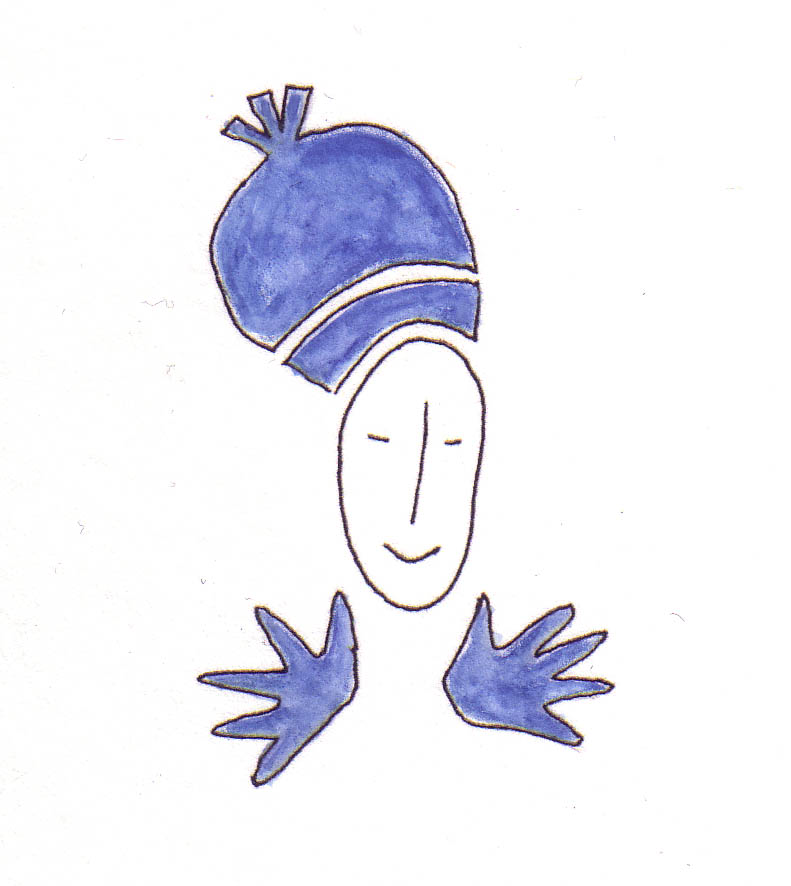
\includegraphics{presentation/img/vasta.png}} \\

- task genereren
- ekskl.pronomen
\textbf{Maid don lohket ikte?} 

Dohkálaš vástádusat:
\begin{itemize}
\item Mun han lohken ollu áviissaid. 
\item Ikte mun gal lohken buori girjji. 
\item In lohkan maidege. 
\item Ikte in lohkan.
\end{itemize}

\textbf{Maid don lohket ikte?} 

Vasta-prográmma bagada go vástádus ii leat dohkálaš:
\begin{itemize}
\item Mun lohket ollu áviissaid. \\ $\rightarrow$ Husk kongruens mellom subjekt og verbal.  
\item Mun lohken ollu áviissat. \\ $\rightarrow$ Objektet skal være i akkusativ. 
\item Don lohket ollu áviissaid. \\ $\rightarrow$ Er du sikker på at du svarer i riktig person?  
\end{itemize}

\subsection{Lunddolaš ságastallan}

\begin{description}
\item [ ] D: Siđat go gáfe?   G: In dieđe vuos.   
\item [ ] $\rightarrow$ Det er for enkelt å svare vet-ikke. Prøv igjen.   
\item [ ] D: Maid háliidat borrat?   G: Láibbi.   
\item [ ] $\rightarrow$ Svaret ditt må alltid inneholde et finitt verb.   
\item [ ] D: Áiggut go vázzit bargui odne?   G: Ale jeara nu olu.   
\item [ ] $\rightarrow$ Er du sikker på at du svarer i riktig person?
\end{description} 



\subsection{Min vuogádat} 
      <text>Maid SUBJ MAINV ikte</text>


\scalebox{0.65}[0.65]{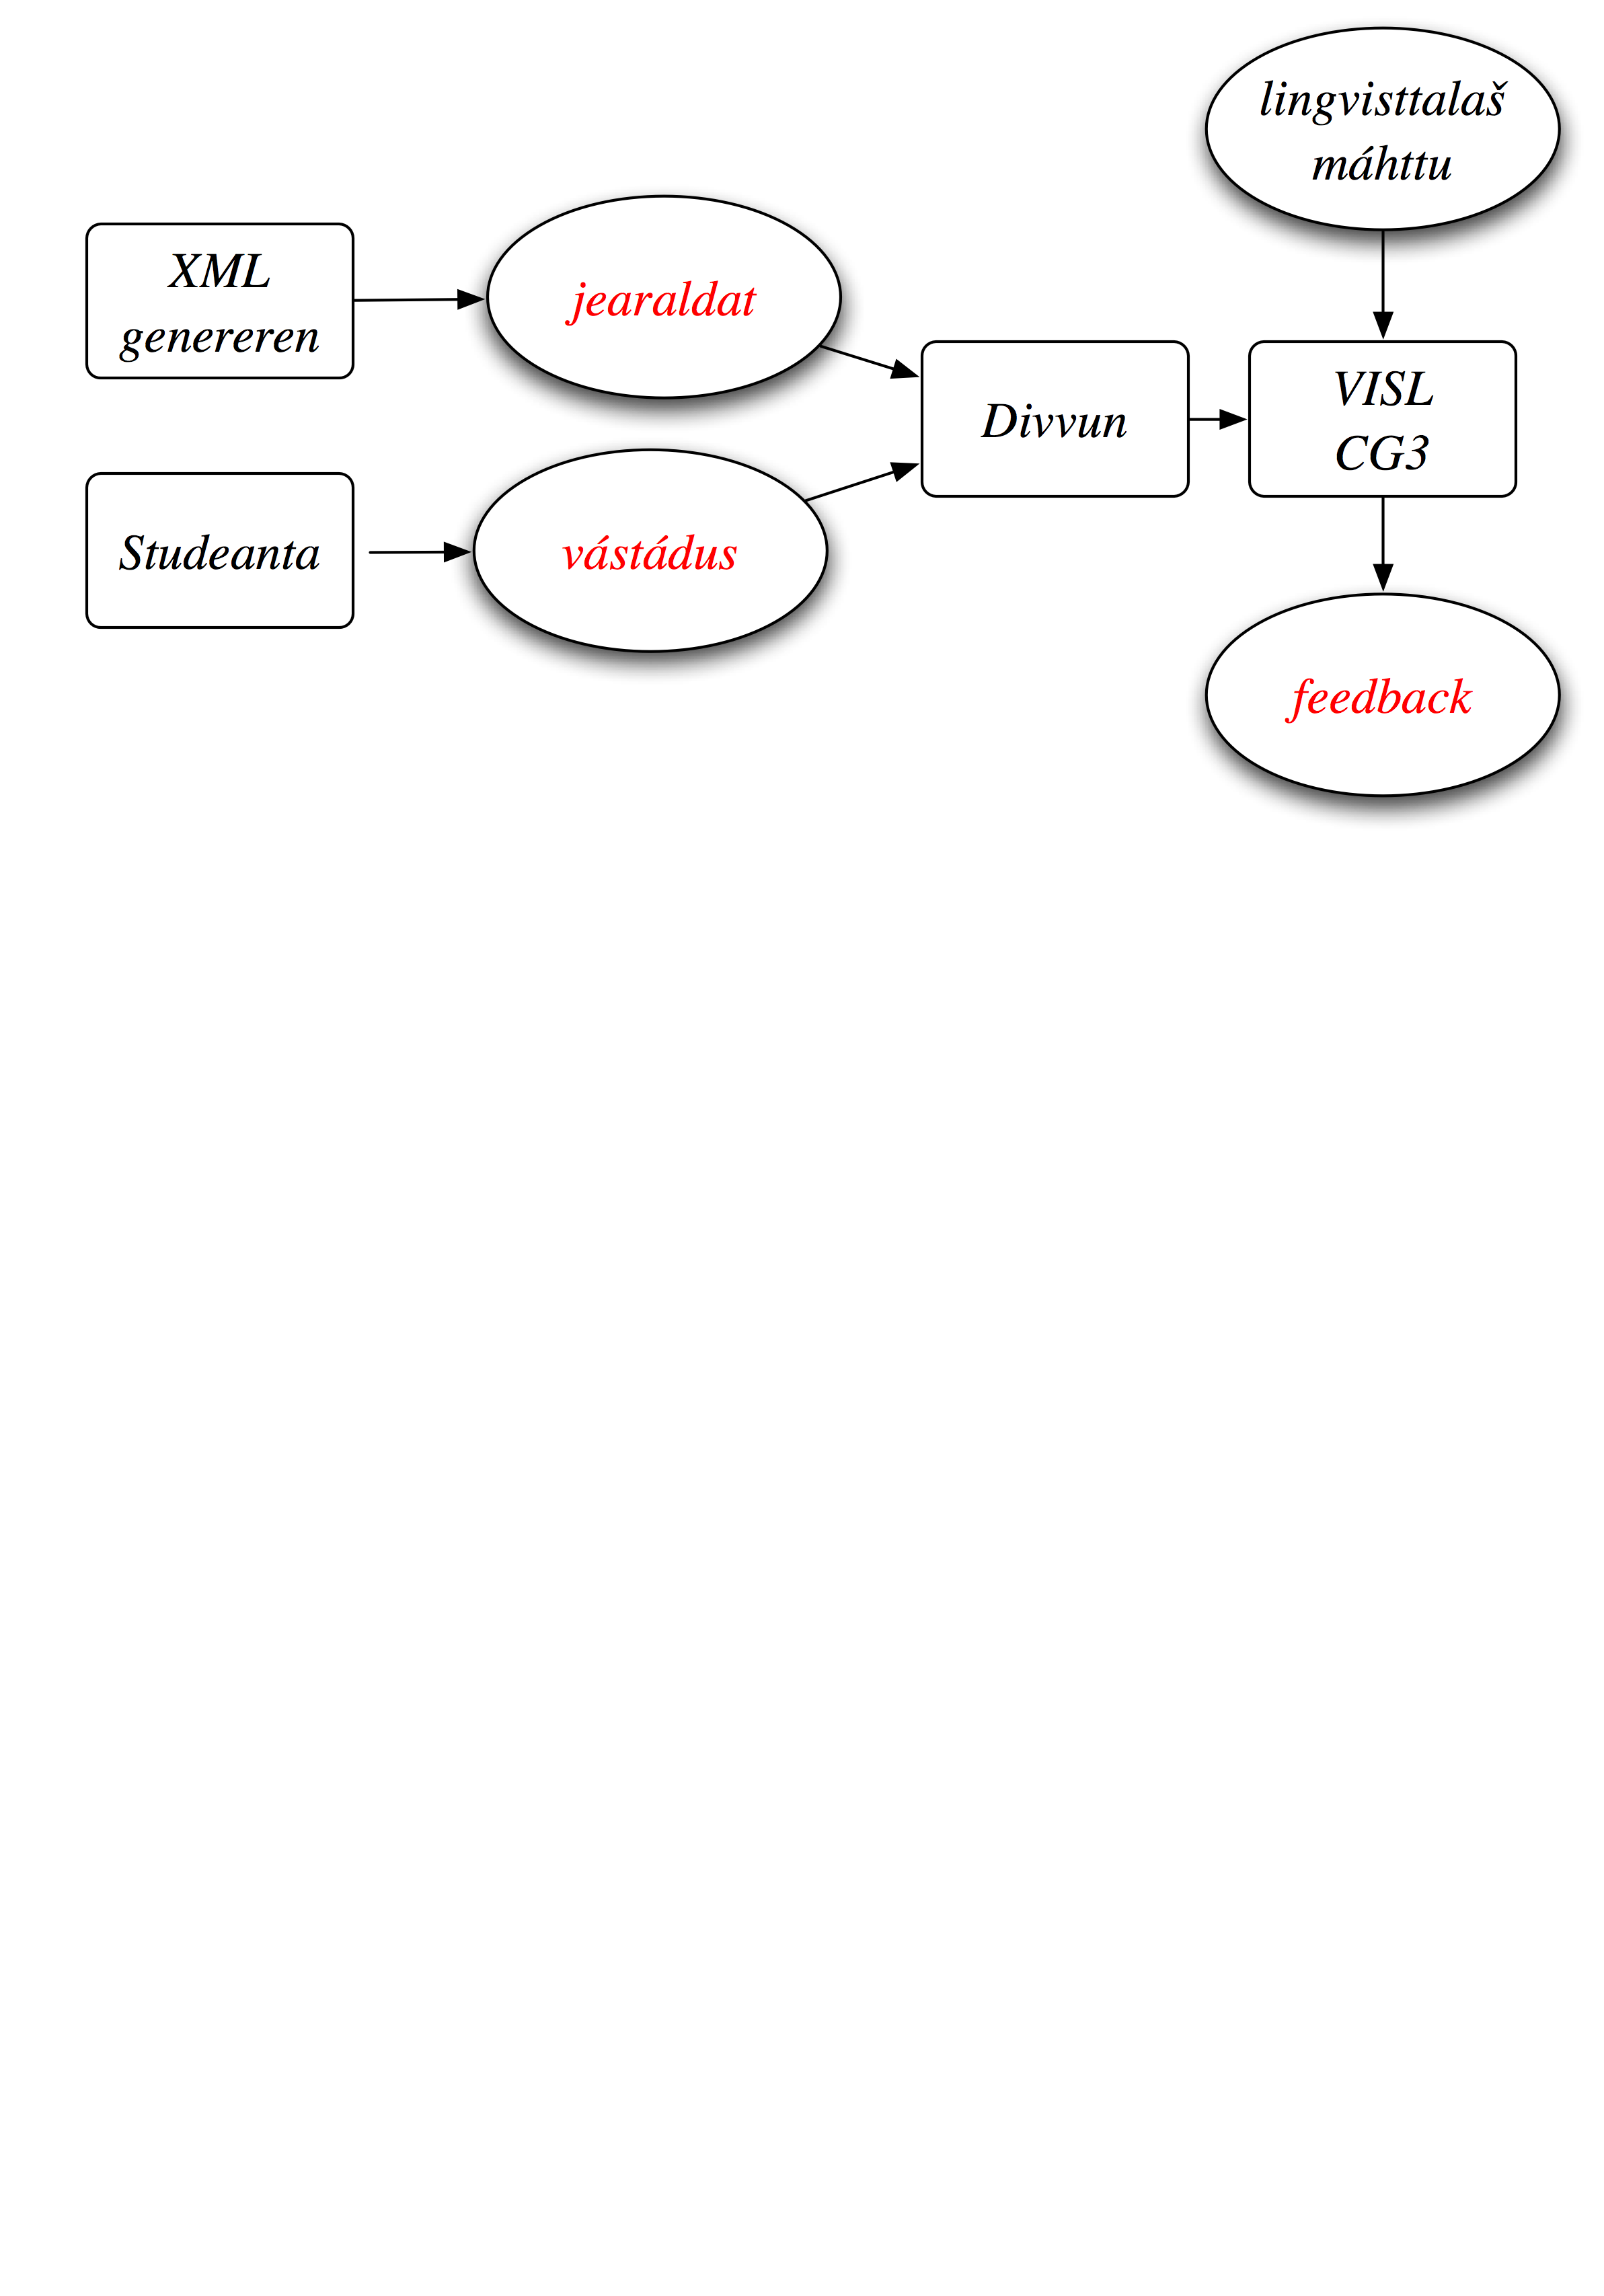
\includegraphics{presentation/img/skovi.png}} 







\subsection{Sahka}
- inklus.pronomen
- čállojuvvon jearaldagat
- no random
- logihkka vástadusa ektui

\begin{figure}[htbp]
\begin{center}
\scalebox{.5}[.5]{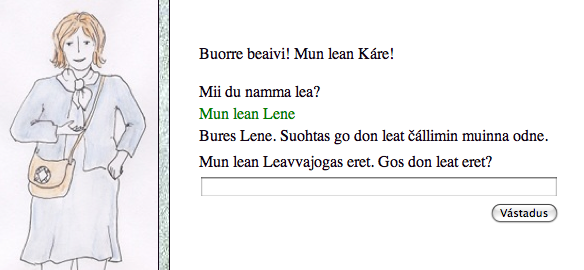
\includegraphics{presentation/img/sahka2.png}}\\
\caption{Sahka, at \textit{http://victorio.uit.no/oahpa/sahka/}}
\label{sahka}
\end{center}
\end{figure}


Scenarios:
\begin{itemize}
\item Get acquainted to Hánsa -- an adult man living in Kautokeino
\item Get acquainted to Káre -- an adult woman living in Karasjok
\item Get acquainted to Lisa -- a girl living in Tana
\item Get acquainted to Lemet -- a boy living in Tromsø
\item Visit -- help to move furniture from one room to another, and have a coffee break
\item Grocery -- buying food
\item Comparing in the shop -- tell what is cheapest or most expensive, using adjectives in comparative or superlative
\end{itemize}


\section{Cuolmmat}
- lunddolaš vai ped?

feedbacka grammatihka vuođul:
- finihtta vearbbat
- nom vs akk

čállinmeattáhusaid bagadeapmi
-----------------------------
- dovdameahttun sátni -
	1. "tastefeil" 
	2. sojahanfeaila
	- álki addit čállinfeailafeedback
	- váttis bagadit geavaheaddji 
		1. gehčosa bokte livččii vejolaš kommenteret
		2. iskat lonuhit a/á 
		3. ped.divvun livččii vejolaš
- áiggukeahtes sátni -
	- váttis addit čállinfeailafeedback
	- vejolaš bagadit
	lok
	ill (báddii)
	biehttalanhápmi
	ordnetlohku vs. Nom.Pl. (viđát vs. viđat)







\subsection{Čuolmmat -- 1}
\textbf{Didaktihkka versus pragmatihkka} \\
Mii háliidit geavaheaddji hárjehallat buot persovnnaid ja loguid. Dan dihte:
\begin{itemize}
\item{Ellipsa ii leat dohkálaš}
\item{Finihtta vearba lea bákkolaš}
\item{Ferte vástidit seammá vearbbain dalle go lea lunddolaš dan dahkat}
\item{Ii leat fátmmasteaddji 1. p duála ja plurála }
\item{\textit{In dieđe} ii leat dohkálaš vástádus}
\end{itemize}

\begin{tabular}[t]{ll|ll|ll}
QPN &APN &QPN &APN &QPN &APN \\
\hline
Sg1 &Sg2 &Du1 &Du2 &Pl1 &Pl2 \\
Sg2 &Sg1 &Du2 &Du1 &Pl2 &Pl1 \\
Sg3 &Sg3 &Du3 &Du3 &Pl3 &Pl3 \\
\hline
\end{tabular}

\begin {itemize}
\item NG (not generate for any of the dialects)
\item NOT-KJ (not generate for KJ-dialect) 
\item NOT-GG (not generate for GG-dialect)  
\end {itemize}


\subsection{Čuolmmat -- 2}
\textbf{Cealkagis ii leat finihtta vearba} \\

\textit{*Mun vuolggan ihttin.}\\
$\rightarrow$ Svaret ditt må alltid inneholde et finitt verb. 

\textbf{Vejolaš čoavddus:}\\

\textit{*Mun vuolggan ihttin.}\\
$\rightarrow$ Svaret ditt må alltid inneholde et finitt verb. Kan det være en skrivefeil?

\subsection{Čuolmmat -- 3}
\textbf{Cealkagis leat guokte finihtta vearbba:} \\
\textit{*Mun áiggun vuolggán.} versus
\textit{Mun boran haman.}\\
-- finihtta-finihtta-konstrukšuvnnas vearbbain galgá leat seammá sojaheapmi\\
-- ii galgga leat advearba gaskkas

\textbf{Vejolaš čoavddus:} \\
Semánttalaš seahtta:\\
LIST INFV = \textit{astat ádjánit áigut álgit beassat berret bivvat ....} \\
\textnormal{Njuolggadus : ii sáhte leat (INFV finihtta) + (VERB finihtta)}

\subsection{Čuolmmat -- 4}
\textbf{Nominatiiva versus akkusatiiva} \\
Eat sáhte luohttit sátneortnegii, ja subjeakta ii leat bákkolaš
\begin{itemize}
\item Jearaldat dáhttu objeavtta (muhto lea dattetge vejolaš vástidit objeavtta haga)
\end{itemize}

\textbf{Vejolaš čoavddus:} \\
Defineret vearbbaid ja bidjat daid semánttalaš seahtaide, omd: 
\begin{itemize}
\item vearbbat main lea objeakta bákkolaš argumeantan  (Strict Transitive Verbs)
\item vearbbat main ii sáhte leat HUMAN objeaktan 
\textit{borrat}   - HUMAN sáhttá leat subjeakta, iige objeakta \\
 
\textit{lohkat}  - seammá, muhto objeakta sáhttá dattetge leat namma, \\ omd   \textit{Ikte mun lohken Fosse.}  \\ 
-- ja de mis lea nubbi mearkkašupmi: \textit{Mun lohken mánáid.}
\end{itemize}


\subsection{Čuolmmat -- 5}
\textbf{Čállinmeattáhusat} \\
\begin{enumerate}
\item sátni ii gávdno: \\ \textit{$\rightarrow$ X finnes ikke i vårt leksikon. Kan det være en skrivefeil?}
\item áiggukeahtes lemma (leksem)
\item rivttes lemma, muhto áiggukeahtes sátnehápmi
\end{enumerate}

\textbf{Kásusgehčosa lasihit njuolgga Nom-hápmái} \\
Min pedleksikonas leat 1512 substantiivva
\begin{itemize}
\item LOKATIIVA -s/-is : \\
57 \% rivttes lemma - áiggukeahtes sátnehápmi (PxSg3 - omd \textit{viessus})  \\  0,5 \% áiggukeahtes lemma \\  (omd. \textit{eanas Adv (eatnamis)}  dahje \\ vearba \textit{-stit} -- imperatiiva, vearbagenetiiva, biehttalanhápmi omd \textit{čogus (čohkumis)} )
\item ILLATIIVA -i/-ii: \\
0 \% rivttes lemma - áiggukeahtes sátnehápmi \\  2,3 \% áiggukeahtes lemma \\ (eanaš Vearba preterihtta Sg3, omd \textit{báddii (báddái)}) 
\end{itemize}


\subsection{Čuolmmat -- 5a}
\textbf{Čállinmeattáhus dahká áiggukeahtes sojaheami} \\
omd oamastangehčosat \\
\textit{biilas N Sg Nom Px Sg3 versus biillas N Sg Loc} \\
\textit{*Áhčči lea biilas.}

\textbf{Vejolaš čovdosat:}
\begin{itemize}
\item Váldit eret oamastangehčosiid, earret dalle go hui čielggas ahte sáhttá leat.
\item Kommenteret geavaheaddjái: \\
$\rightarrow$ Mener du lokativ? I så fall er det feil stadieveksling.
\end{itemize}

\subsection{Čuolmmat -- 5b}
\textbf{Čállinmeattáhus dahká áiggukeahtes lemma} \\
\begin{itemize}
\item \textit{viessut:  viessut} Inf dahje \textit{viessat} Imprt \\
muhto čálli dáidá oaivvildit \textit{viesut} N Pl Nom.   
\item \textit{luomos}: A Attr \\
\textit{*Eadni lea luomos.} \\
$\rightarrow$ Her skulle det ikke vært attributtform. \\  
\textit{Gos eadni lea?} \\ 
$\rightarrow$ Svaret burde inneholde en lokativ.
\end{itemize}

\textbf{Vejolaš čovdosat:}
\begin{itemize}
\item Váldit eret problemáhtalaš lemmaid dahje sátnehámiid
\item Identifiseret sátnebáraid ja jearrat geavaheaddjis: \\ $\rightarrow$ Mener du viessu = hus? I så fall er det feil stadieveksling.
\end{itemize}




\subsection{Divvut vai ii}
\textbf{Buoret ahte soames áššit báhcet divukeahttá go divvut dakkára mii leat riekta}
- muhto duhtágo geavaheaddji dasa?

\subsection{Evalueren ja buorideapmi}
\begin{itemize}
\item Responsa geavaheddjiin
\item Responsa oahpaheddjiin
\item Ráhkadit vástáduskorpusa (Vasta-log interneahtas)
\end{itemize}

\section{vejolašvuođat ja konklušuvdna}
- semantalaš rollat? \\
boahtteáiggis: diehtovuorká ? \\
Oahpa-divvun-systema ? \\
Sámediggi ja Romssa Universitehta leat ruhtadan barggu


\newpage

%\begin{spacing}{1}
\par
%\bibliographystyle{jmr} %jmr gives the second author with first name first
\bibliographystyle{jmr}
\bibliography{WAart}
\addcontentsline{toc}{section}{References}
%\end{spacing}


\end{document}

